\documentclass[11pt]{article}
\usepackage{amssymb}
\usepackage{amsthm}
\usepackage[fleqn]{amsmath}
\usepackage{listings}
\usepackage{color}
\usepackage{graphicx}
\usepackage{subcaption}
\usepackage[margin=1.0in]{geometry}

\lstdefinestyle{matlab-style}{
language=Matlab,
basicstyle=\scriptsize\ttfamily,
tabsize=2,
rulecolor=,
language=matlab,
basicstyle=\scriptsize,
aboveskip={1.5\baselineskip},
columns=fullflexible,
showstringspaces=false,
extendedchars=true,
breaklines=true,
prebreak = \raisebox{0ex}[0ex][0ex]{\ensuremath{\hookleftarrow}},
frame=single,
showtabs=false,
showspaces=false,
showstringspaces=false,
identifierstyle=\ttfamily,
keywordstyle=\color[rgb]{0,0,1},
commentstyle=\color[rgb]{0.133,0.545,0.133},
stringstyle=\color[rgb]{0.627,0.126,0.941},
keepspaces=true,
numbers=left,
numbersep=5pt,
numberstyle=\tiny\color[rgb]{0.5,0.5,0.5},
stepnumber=1
}

\newcommand{\bs}[1] {\boldsymbol{#1}}

\title{Mandating fun on a tilt-o-whirl\\MANE 6963 - Project 3}
\author{ID: 2168}
\date{}

\begin{document}

\maketitle

\section{Executive summary}

In this report, we investigate the optimal design of a
tilt-o-whirl amusement ride, where riders' cars spin
independently about a platform, while also spinning
about a central platform. Our objective is to maximize
the standard deviation of the angular velocity of each
car on the platform, which is thought to increase
the unpredictability and thus fun of the ride.

\begin{figure}[hbt!]
\centering
\begin{subfigure}{.25\textwidth}
\centering
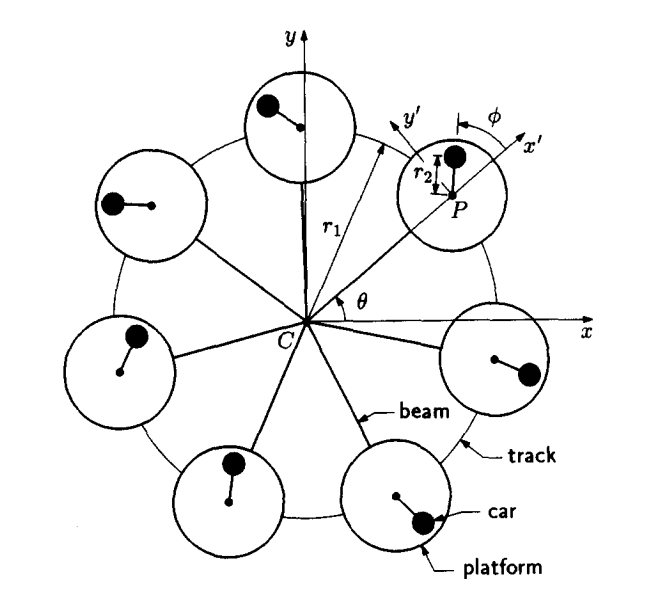
\includegraphics[width=.99\linewidth]{ride1}
\end{subfigure}%
\begin{subfigure}{.25\textwidth}
\centering
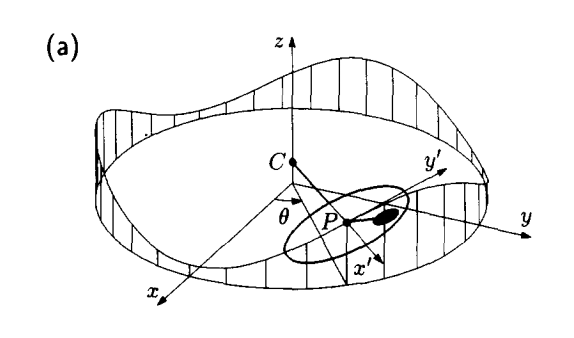
\includegraphics[width=.99\linewidth]{ride2}
\end{subfigure}%
\begin{subfigure}{.25\textwidth}
\centering
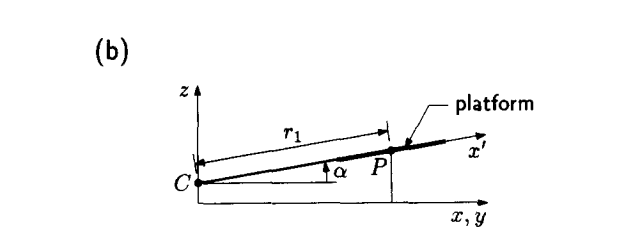
\includegraphics[width=.99\linewidth]{ride3}
\end{subfigure}%
\begin{subfigure}{.25\textwidth}
\centering
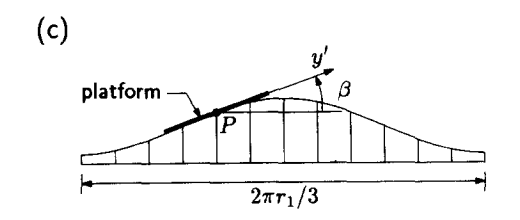
\includegraphics[width=.99\linewidth]{ride4}
\end{subfigure}
\caption{Tilt-o-whirl ride diagrams}
\label{fig:ride}
\end{figure}

\section{Analysis methods}

\subsection{Analysis verification}

\section{Optimization methods}

\section{Results}

\begin{verbatim}
 Norm of First-order
 Iter F-count            f(x) Feasibility  Steplength        step  optimality
    0       4   -1.488281e+00   0.000e+00                           1.364e+01
    1       8   -2.126049e+00   0.000e+00   1.000e+00   4.781e-01   1.013e+01
    2      14   -2.175085e+00   0.000e+00   4.900e-01   3.790e-01   6.000e+00
    3      18   -2.732151e+00   0.000e+00   1.000e+00   4.389e-01   5.211e+00
    4      22   -4.702722e+00   2.776e-17   1.000e+00   5.857e-01   7.417e+00
    5      28   -4.731514e+00   1.388e-17   4.900e-01   7.872e-02   4.500e+00
    6      39   -4.812858e+00   0.000e+00   8.235e-02   8.437e-02   2.863e+00
    7      47   -4.816365e+00   0.000e+00   2.401e-01   3.087e-02   3.659e+00
    8      53   -4.822389e+00   0.000e+00   4.900e-01   6.119e-02   2.798e+00
    9      59   -4.894551e+00   0.000e+00   4.900e-01   5.556e-02   3.447e+00
   10      63   -4.928094e+00   0.000e+00   1.000e+00   2.138e-02   7.479e-01
   11      67   -4.931250e+00   0.000e+00   1.000e+00   4.901e-03   4.142e-01
   12      71   -4.932860e+00   0.000e+00   1.000e+00   7.100e-03   1.354e-01
   13      75   -4.932945e+00   0.000e+00   1.000e+00   1.270e-03   3.173e-02
   14      79   -4.932950e+00   0.000e+00   1.000e+00   2.553e-04   1.613e-03
   15      83   -4.932950e+00   0.000e+00   1.000e+00   1.574e-05   4.258e-04
   16      87   -4.932950e+00   0.000e+00   1.000e+00   3.167e-06   2.909e-05
   17      91   -4.932950e+00   0.000e+00   1.000e+00   4.304e-07   4.768e-06
\end{verbatim}

\begin{verbatim}
p =

    0.7760    0.1762    0.2261

>> (1.488281-4.932950)/1.488281

ans =

   -2.3145
\end{verbatim}

\section{Conclusion}

\section{Math}

\begin{equation}
\frac{d}{d \tau}
\begin{bmatrix}
y_1\\
y_2
\end{bmatrix}
=
\begin{bmatrix}
F(y_1, y_2) \\
y_1
\end{bmatrix},
\end{equation}
%
where
%
\begin{equation}
F(y_1, y_2) =
(\gamma / Q_0) y_1 +
(\epsilon - \gamma^2 \alpha) \sin (y_2) +
\gamma^2 \beta \cos(y_2),
\end{equation}
%
and the following variables are defined as:
$y_1 = \frac{d \phi}{d \tau}$, $y_2 = \phi$,
$\alpha = \alpha_0 - \alpha_1 \cos \tau$,
$\beta = 3 \alpha_1 \sin \tau$,
$\epsilon = \frac{r_1}{9 r_2}$,
$\gamma = \frac{1}{3 \omega} \sqrt{g / r_2}$.

\end{document}
